\chapter{Introduction} \label{chap:intro}


%###############################################################################################################################
%###############################################################################################################################
%###############################################################################################################################
\section{Nuclear Fusion}%
\label{sec:intro_whatisfusion}

Nuclear fusion is a reaction which combines multiple light nuclei together into heavier nuclei.
If the products of the reaction are more tightly bound than the reactants, excess energy is also released to the products.
Broadly, the binding energy per nucleon of common nuclear isotopes increases with atomic mass up to iron, ${}^{56}\text{Fe}$, and decreases afterwards, as is shown in Fig.~\ref{fig:intro_BEperNucleon}.
The reverse process, nuclear fission, operates by splitting heavy nuclei into lighter products, thus energy is released via fusion by combining elements up to iron and via fission down to iron.
In 2023, fission made up approximately 9.1\% of the global electricity mix~\cite{ember_institute_statistical_2024}.
Like fission, fusion energy would be carbon free at the point of production, but it would also offer further distinct advantages.
Fusion power plants would not produce energy via potentially dangerous chain reactions and would generate little-to-no long-lived nuclear waste, depending on the specific fuel that was used.
In comparison with other low-carbon power sources, including wind and solar, studies have shown that fusion energy could have a competitive \ac{LCOE}, which is a metric that compares the economic costs of a power plant over its lifetime to the value of energy produced~\cite{griffiths_commercialisation_2022}.
Performing controlled nuclear fusion on Earth for energy production has been an active area of research for many decades and many significant scientific and engineering challenges remain to be resolved, in order to make it a viable energy source.

The likelihood of two reactants undergoing a specific fusion reaction is described by the cross-section of the interaction,
\begin{equation}
    \label{eq:intro_cross_sec}
    \sigma(E) = \frac{S(E)}{E} e^{-E_G/E},
\end{equation}
which is a function of the centre of mass energy, $E$, the `astrophysical $S$-factor', $S(E)$, which is a weakly varying function of energy for many typically deployed reactants and the Gamow Energy, $E_G$~\cite{atzeni_physics_2004}.
The exponential term in Eq.~\ref{eq:intro_cross_sec} is related to the probability of reactants tunnelling through the energy barrier, due to electrostatic Coulomb repulsion.
One approach to achieving the energies required to overcome this barrier are `beam-target' configurations, wherein a high energy beam of reactants is focussed onto a stationary target, has proven unviable~\cite{rider_general_1995}.
Thermonuclear fusion is the alternative approach, wherein the bulk fuel is heated to sufficient temperatures that the particles in the high-energy tail of the distribution have sufficient energy to undergo fusion reactions.
For a fuel is in thermal equilibrium, the high particle energies required to overcome the Coulomb barrier, $\mathcal{O}(100)\ \text{keV}$, are well above ionisation energies, $13.6\ \text{eV}$ for Hydrogen, so the fuel will be in the plasma state.
If the fusion products are able to deposit a sufficient fraction of their energy back into the fuel, then a self-sustaining fusion reaction is possible, where the high temperatures required for the reactants to fuse is maintained.
For a fusion reaction with reactants labelled by 1 and 2, the number of fusion reactions per unit time and volume is known as the `volumetric reaction rate',
\begin{equation}
    \label{eq:intro_reacrate}
    R_{12} = \frac{n_1 n_2}{1+\delta_{12}} \langle \sigma v \rangle,
\end{equation}
where $v$ is the relative velocity of a pair of reactants, $\delta_{12}$ is the Kronecker delta, which accounts for double counting of species and the `averaged reactivity' $\langle \sigma v \rangle$ is defined as the integral over the velocity distribution,
\begin{equation}
    \label{eq:intro_reactivity}
    \langle \sigma v \rangle \equiv \int_0^{\infty} \sigma(E) v f(v)\ \text{d}v.
\end{equation}
Eq.~\ref{eq:intro_reacrate} explicitly demonstrates that achieving a high fuel density, can significantly enhance reaction rates due to the square dependence.

\begin{figure}[t!]
    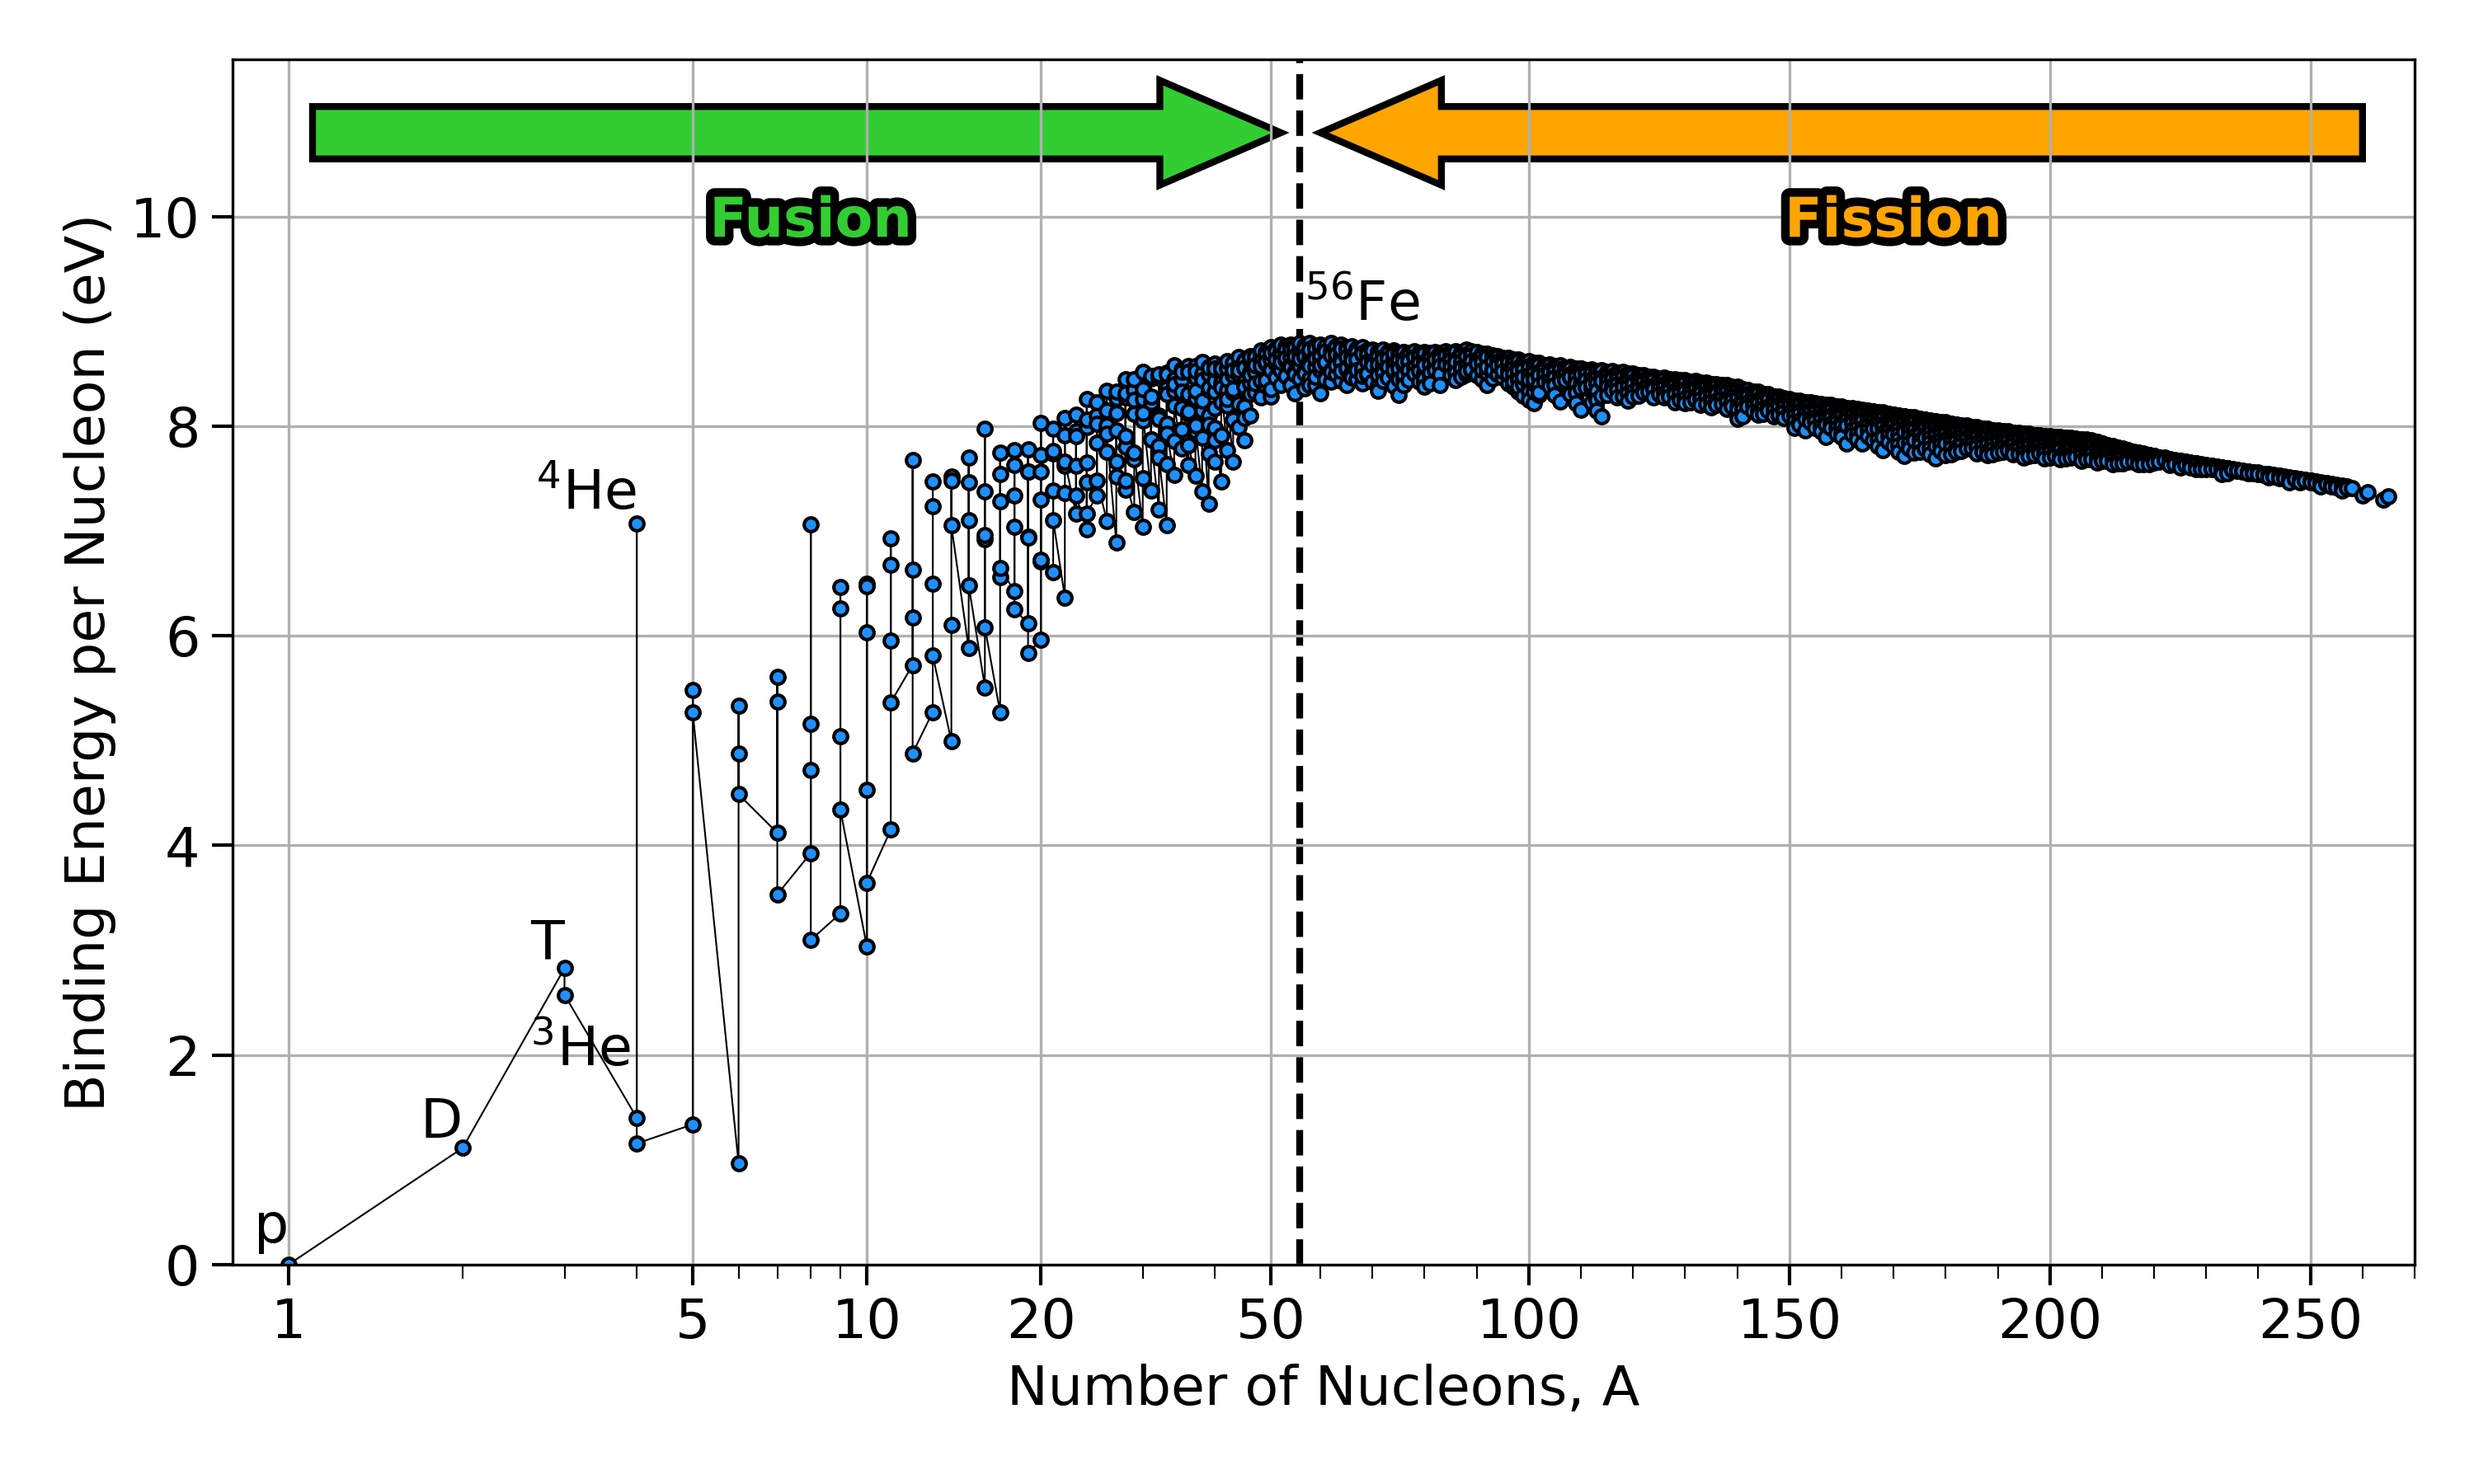
\includegraphics[width=0.9\linewidth]{Introduction/Images/BE_per_nucleon.png}
    \centering
    \caption{Binding energy per nucleon for common nuclear isotopes.
    Binding energy peaks close to iron, therefore energy is released for reactions which increase binding energy.
    ${}^{4}\text{He}$ has a particularly high binding energy and therefore fusion reactions which results in this isotope are strong candidates for fusion energy production.}%
    \label{fig:intro_BEperNucleon}
\end{figure}

\begin{figure}[t!]
    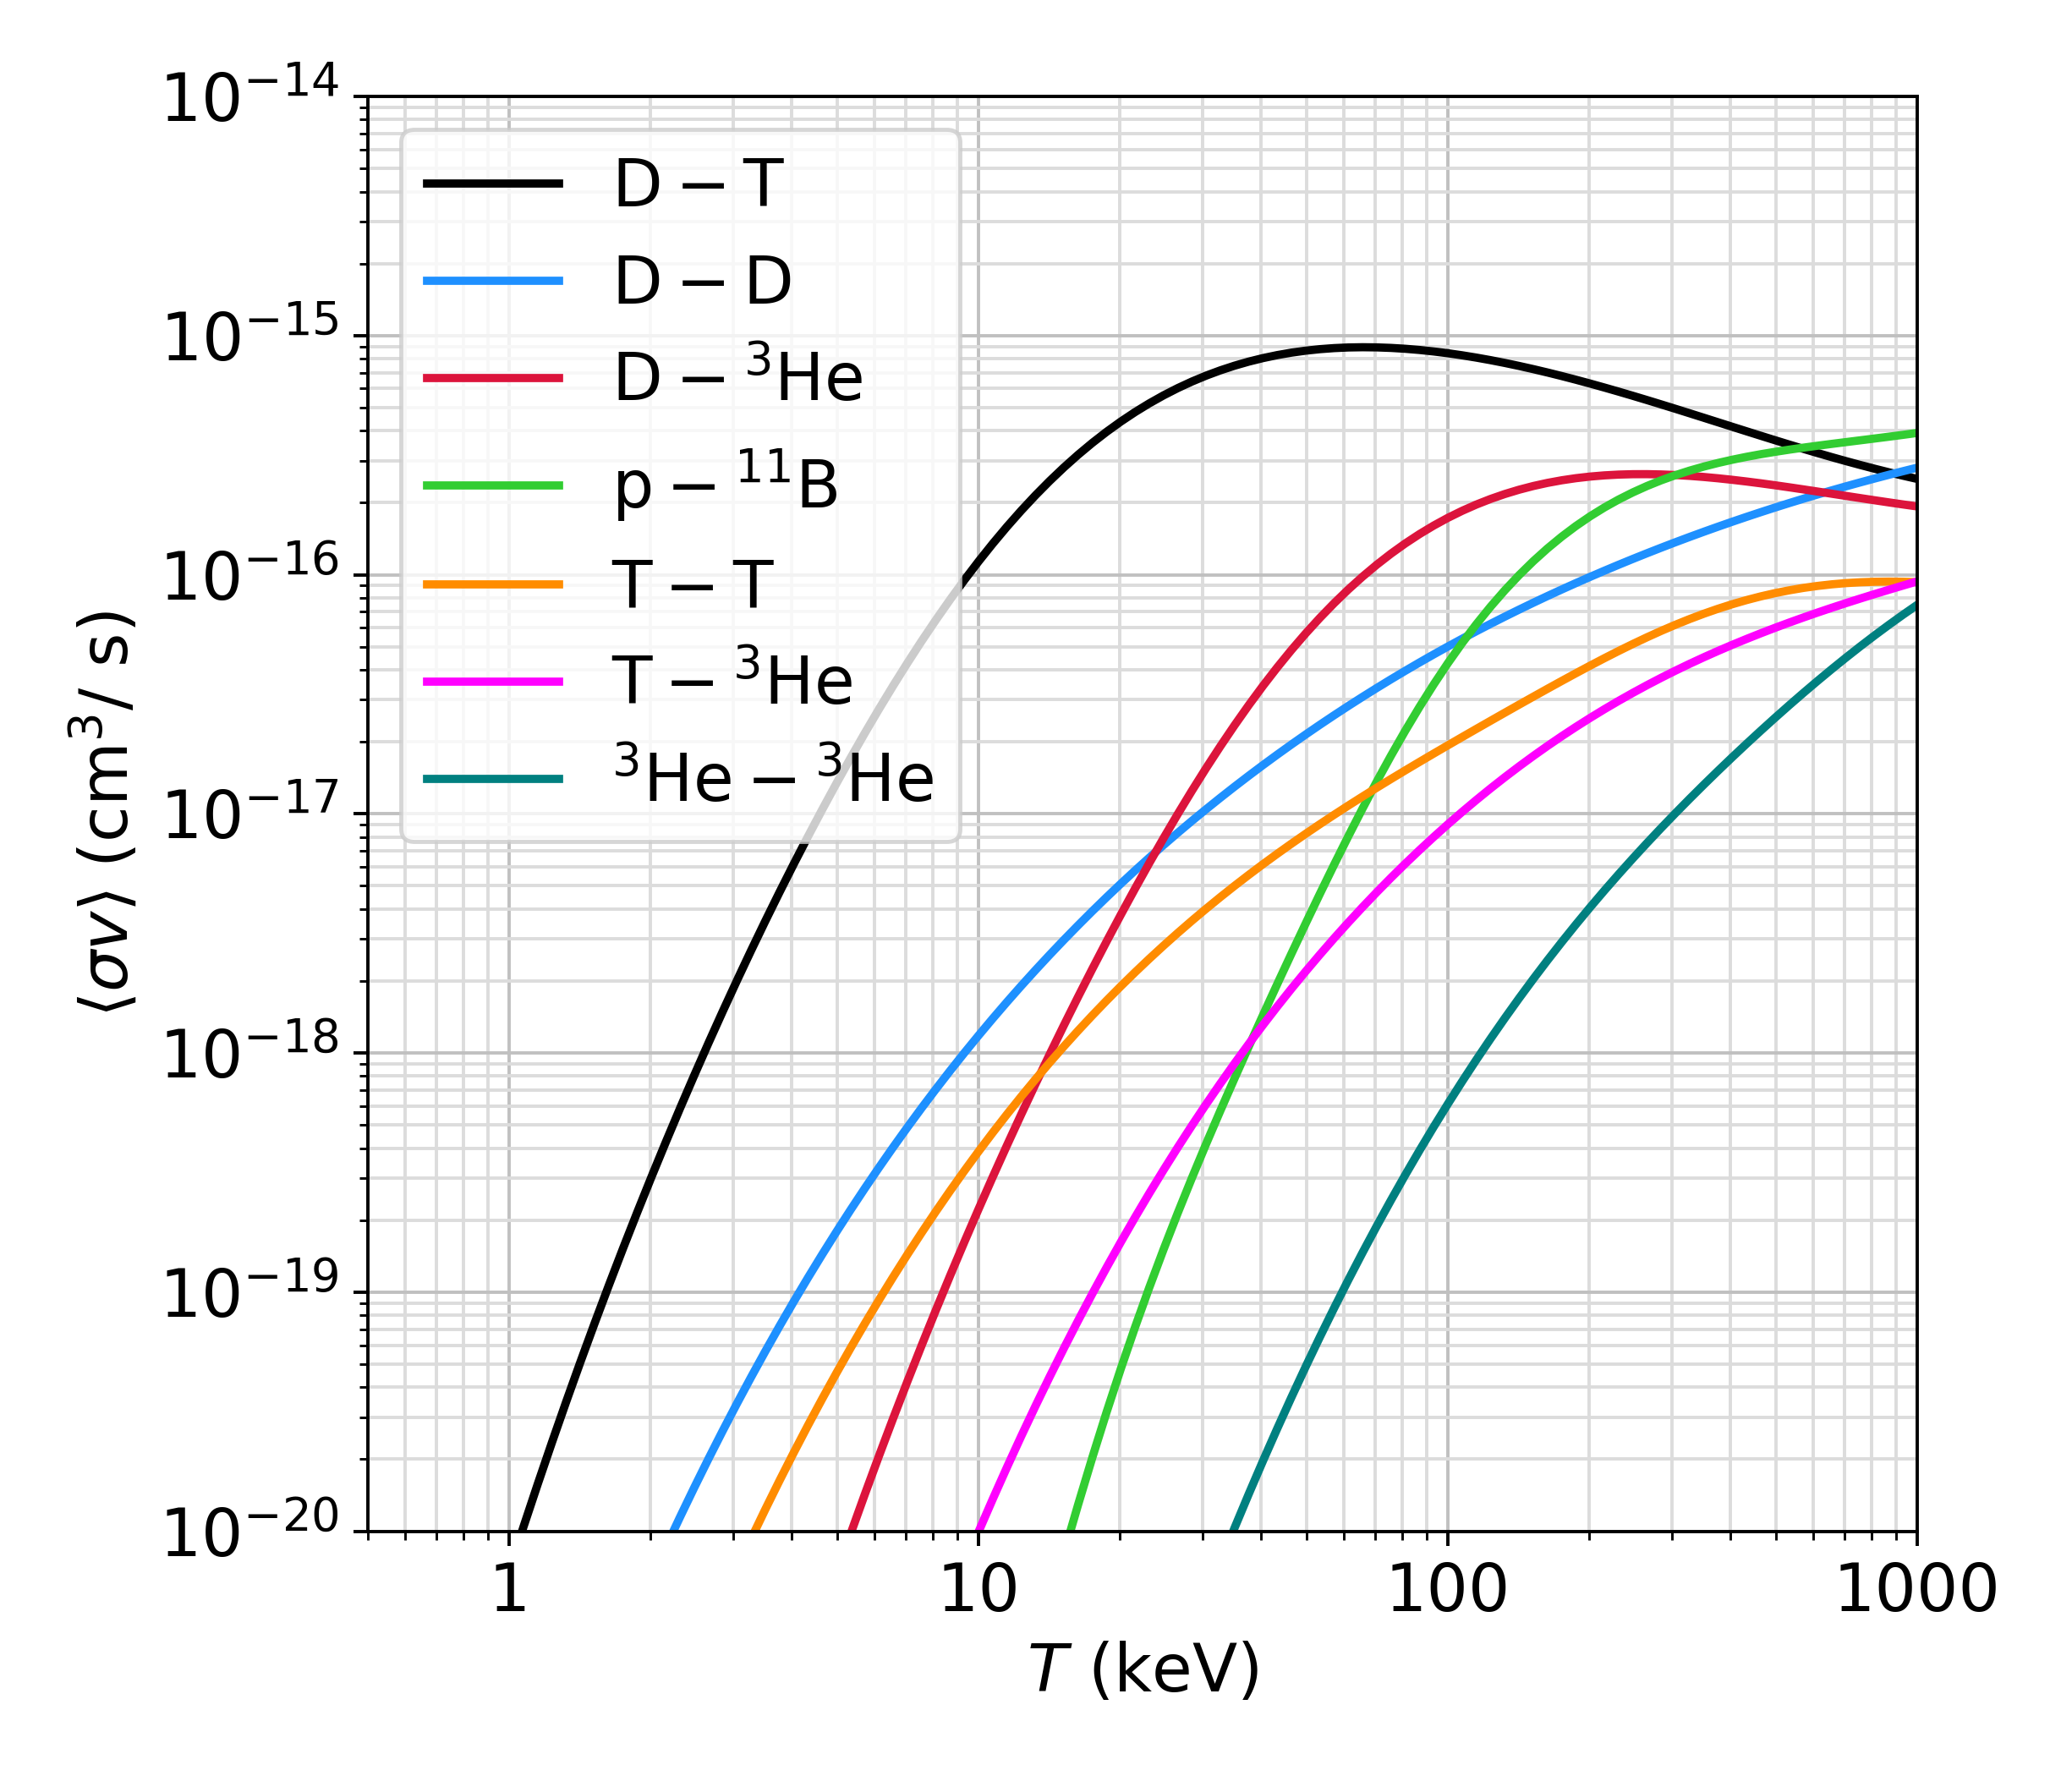
\includegraphics[width=0.6\linewidth]{Introduction/Images/fusion-reactivities.png}
    \centering
    \caption{Averaged reactivities for important fusion reactions.
    The deuterium-tritium reactivity is significantly larger than all other reactions up to $T\sim500\ \text{keV}$.
    Averaged reactivities are obtained from cross-section data, available in the \texttt{ENDF/B-VII.1} library~\cite{chadwick_endfb-vii1_2011}.
    }%
    \label{fig:intro_reactivities}
\end{figure}

The efficacy of a fusion fuel is dictated by the availability of the reactants, the fusion products, the averaged reactivity of the reactants and the energy released per reaction, $Q$, which is the difference in binding energy between the reactants and products.
Most current, fusion-energy experiments are focussed on demonstrating that fusion power production is possible, thus the choice of fuel is predominantly dictated by the reactivity.
Hydrogen-Hydrogen isotope fusion reactions have much higher reactivities than other elements, because the Coulomb repulsion scales as $Z^2$, thus the Gamow energy, $E_G$ is significantly smaller.
The nuclear physics is particularly favourable for the fusion of deuterium (D) and tritium (T), because there is a nuclear resonance at relatively modest energies for the reaction chain which produces an excited, unstable ${}^5 \text{He}$ nucleus, which subsequently decays to ${}^4\text{He}$ and a neutron~\cite{brown_field_2014}.
Averaged-reactivates of several important fusion reactions, obtained from reaction cross-sections from the \texttt{ENDF/B-VII.1} library~\cite{chadwick_endfb-vii1_2011}, are plotted in Fig.~\ref{fig:intro_reactivities}.
The D-T reactivity is at least an order of magnitude larger than the other reactions plotted, up to $T\sim100\ \text{keV}$, and it is thus the most commonly used fuel for high-gain fusion experiments.
The reaction proceeds as,
\begin{equation}
    \label{eq:intro_DTreac}
    {}^{2}_{1}\text{D} + {}^{3}_{1}\text{T} \rightarrow \alpha(3.5\ \text{MeV}) + \text{n}(14.1\ \text{MeV}),
\end{equation}
where $\alpha$ is a ${}^{4}_{2}\text{He}$ nucleus, which gains $3.5\ \text{MeV}$, and $\text{n}$ is a neutron, which gains $14.1\ \text{MeV}$ from the fusion energy released, $Q$.
The energy partition is dictated by energy-momentum conservation of the products in the centre of mass frame.
The alpha particles typically couple their energy back into the bulk fuel via Coulomb collisions, which has the effect of raising the fuel temperature and thus further raising the reactivity, for fuel temperatures below $T\sim60\ \text{keV}$.
Neutrons have a much lower reaction cross-section because they are not charged, and thus typically leave the reaction region.
However, in fusion experiments with high density configurations such as \ac{ICF}, their heating of the fuel can also play a significant role~\cite{daughton_influence_2023}.

In order for net energy gain, sufficient energy must be released by fusion to compensate for the energy required to perform the experiment.
This requires a fuel configuration with a combination of high temperatures and densities for a large volumetric reaction rate, that is confined for a period of time, which is sufficient for enough reactions to occur.
The method of confinement for fusion energy experiments has two broad streams: \ac{MCF}, where magnetic fields are used to confine steady-state fusion-plasma over long time-scales, and \ac{ICF}, where dense fusion fuel is assembled for a short time period and `confined' by its own inertia.
The work conducted in this thesis is of relevance to \ac{ICF} schemes, specifically those in which the plasma is produced by laser irradiation.

%###############################################################################################################################
%###############################################################################################################################
%###############################################################################################################################
\section{Inertial Confinement Fusion}%
\label{sec:intro_ICF}

In the 1950s and 60s, the first devices were built which demonstrated stimulated emission of microwave~\cite{schawlow_infrared_1958} and optical~\cite{maiman_stimulated_1960} light.
The optical-wavelength lasers were quickly recognised as an ideal driver for a far smaller and therefore less destructive thermonuclear device than was used in warheads, which could thus be used for fusion energy generation~\cite{nuckolls_early_1998}.
Much of the research was declassified and subsequently published in a 1972 article by Nuckolls \textit{et al.} in 1972~\cite{nuckolls_laser_1972}.
In these \ac{ICF} experiments, the high temperatures and densities required to initiate an appreciable number of fusion reactions are maintained over a short timescale, which is set by the inertia of the fuel configuration, before the fuel disassembles due to large pressure gradients.
The required fuel density is typically achieved by an implosion process.
High temperatures are typically obtained either from the conversion to internal energy of the implosion kinetic energy, which is the central hotspot ignition variant, described in Sec.~\ref{sec:intro_centralhotspot}, or via an external heating source, as described in Sec.~\ref{sec:intro_icf_alt}.
Before describing these schemes in more detail however, necessary criterion for energy gain conditions shall be discussed, which are agnostic of how the fusion fuel is assembled and dictate the plasma conditions which must be achieved.

%################################################################################
%################################################################################
\subsection{Ignition Requirements}%
\label{sec:intro_icf_ignition}

The point at which alpha heating becomes the dominant term in the power balance of the fusion fuel is termed `ignition' and it is a necessary condition for high gain \ac{ICF} experiments.
Ignition necessitates that the plasma is confined for a sufficiently long period of time, for an appreciable number of fusion reactions to occur, raising the fuel temperatures and reactivities, which results in a propagating burn wave.
Estimates for the required plasma conditions which must be achieved for this to occur, can be estimated by considering the timescales of confinement and fusion.
Initially, a uniform ion number density $n_i$ and temperature $T$, spherical fuel assembly, with outer radius $R$, shall be considered.
The ions have an average mass, $m_i$, such that the mass-density of the fuel, $\rho = m_i n_i$ and the volume of the fuel sphere, $V = 4\pi R^3/3$.
Dimensional considerations give an order of magnitude estimate for the timescale on which fusion reactions occur,
\begin{equation}
    \tau_{\text{fus}} = \frac{1}{n_i \langle \sigma v \rangle},
\end{equation}
where $n_i$ in the ion number density of the plasma.
A radially inward pressure gradient will exist due to the high temperature of the plasma, which will lead to an inward propagating rarefaction wave, disassembling the fuel.
This rarefaction wave will move at the isothermal sound speed, $c_s=\sqrt{2k_{\text{B}T/m_i}}$,\footnote{The factor of 2 in $C-s$ is because the pressure is the sum of contributions from ions and electrons.} from $t=0$, such that its position is given by $r=R-c_s t$.
Therefore, the timescale on which the burning fuel remains un-rarefied and thus confined is,
\begin{align}
    \begin{split}
        \tau_{\text{conf}} &= \int_0^{R/c_s} \frac{ (R - c_s t)^3 }{R^3} \ \text{d}t,\\
        &= \frac{R}{4 c_s}.
    \end{split}
\end{align}
The ratio of these timescales,
\begin{equation}
    \frac{\tau_{\text{conf}}}{\tau_{\text{fus}}} = \frac{\langle \sigma v \rangle \rho R}{4 m_i c_s},
\end{equation}
illustrates that, for ignition and hence gain, \ac{ICF} reactions require a large $\rho R$ value, which is typically referred to as the `areal-density'~\cite{fraley_thermonuclear_1974}.

The timescale ratio can be used to derive the `burn-up fraction', which is defined as the ratio of fusion reactions, $N_{\text{fus}} = R_{\text{DT}}V\tau_{\text{conf}}$, to the number of DT pairs, $N_{\text{DT}}=n_i/2$, in the fuel assembly,
\begin{align}
    \label{eq:intro_burn_frac}
    \begin{split}
        \Phi &\equiv \frac{N_{\text{fus}}}{N_{\text{DT}}},\\
        &= \frac{\langle \sigma v \rangle \rho R}{H_{\text{B}}},
    \end{split}
\end{align}
where the `burn-parameter', $H_{\text{B}} \equiv \langle \sigma v \rangle / 8 m_i c_s$ has been defined.
Eq.~\ref{eq:intro_burn_frac} is only valid for $\Phi \ll 1$, because the conversion of DT pairs into non-fusing products has not been considered~\cite{atzeni_physics_2004}.
A modified form of Eq.~\ref{eq:intro_burn_frac}, which approximately accounts for burn-depletion, was derived by Fraley \textit{et al.} in Ref.~\cite{fraley_thermonuclear_1974},
\begin{equation}
    \Phi = \frac{\rho R}{H_{\text{B}} + \rho R}.
\end{equation}
If solid density DT was used, the mass of fuel required to achieve $\Phi=30\%$ of the fuel would be 2.5 kg, which would release the same energy as 50 kilotons of TNT~\cite{crilly_simulation_2020}.
In order to harness the released fusion energy without destroying the surrounding infrastructure, a smaller mass is required, which necessitates compression of the fuel to achieve the $\rho R$ constraint.
A pellet containing $1\ \text{mg}$, compressed to densities $\mathcal{O}(10^3)$ times solid density, could release $100\ \text{MJ}$ of fusion energy at $\Phi=30\%$.
Spherical compression is optimal because the fuel compresses in three dimensions.
This minimises the convergence ratio, $CR = R_{\text{init}}/R_{\text{final}}$, which increases the tolerance to a given amplitude of perturbation.

%################################################################################
%################################################################################
\subsection{Central Hotspot Ignition}%
\label{sec:intro_centralhotspot}

\begin{figure}[t!]
    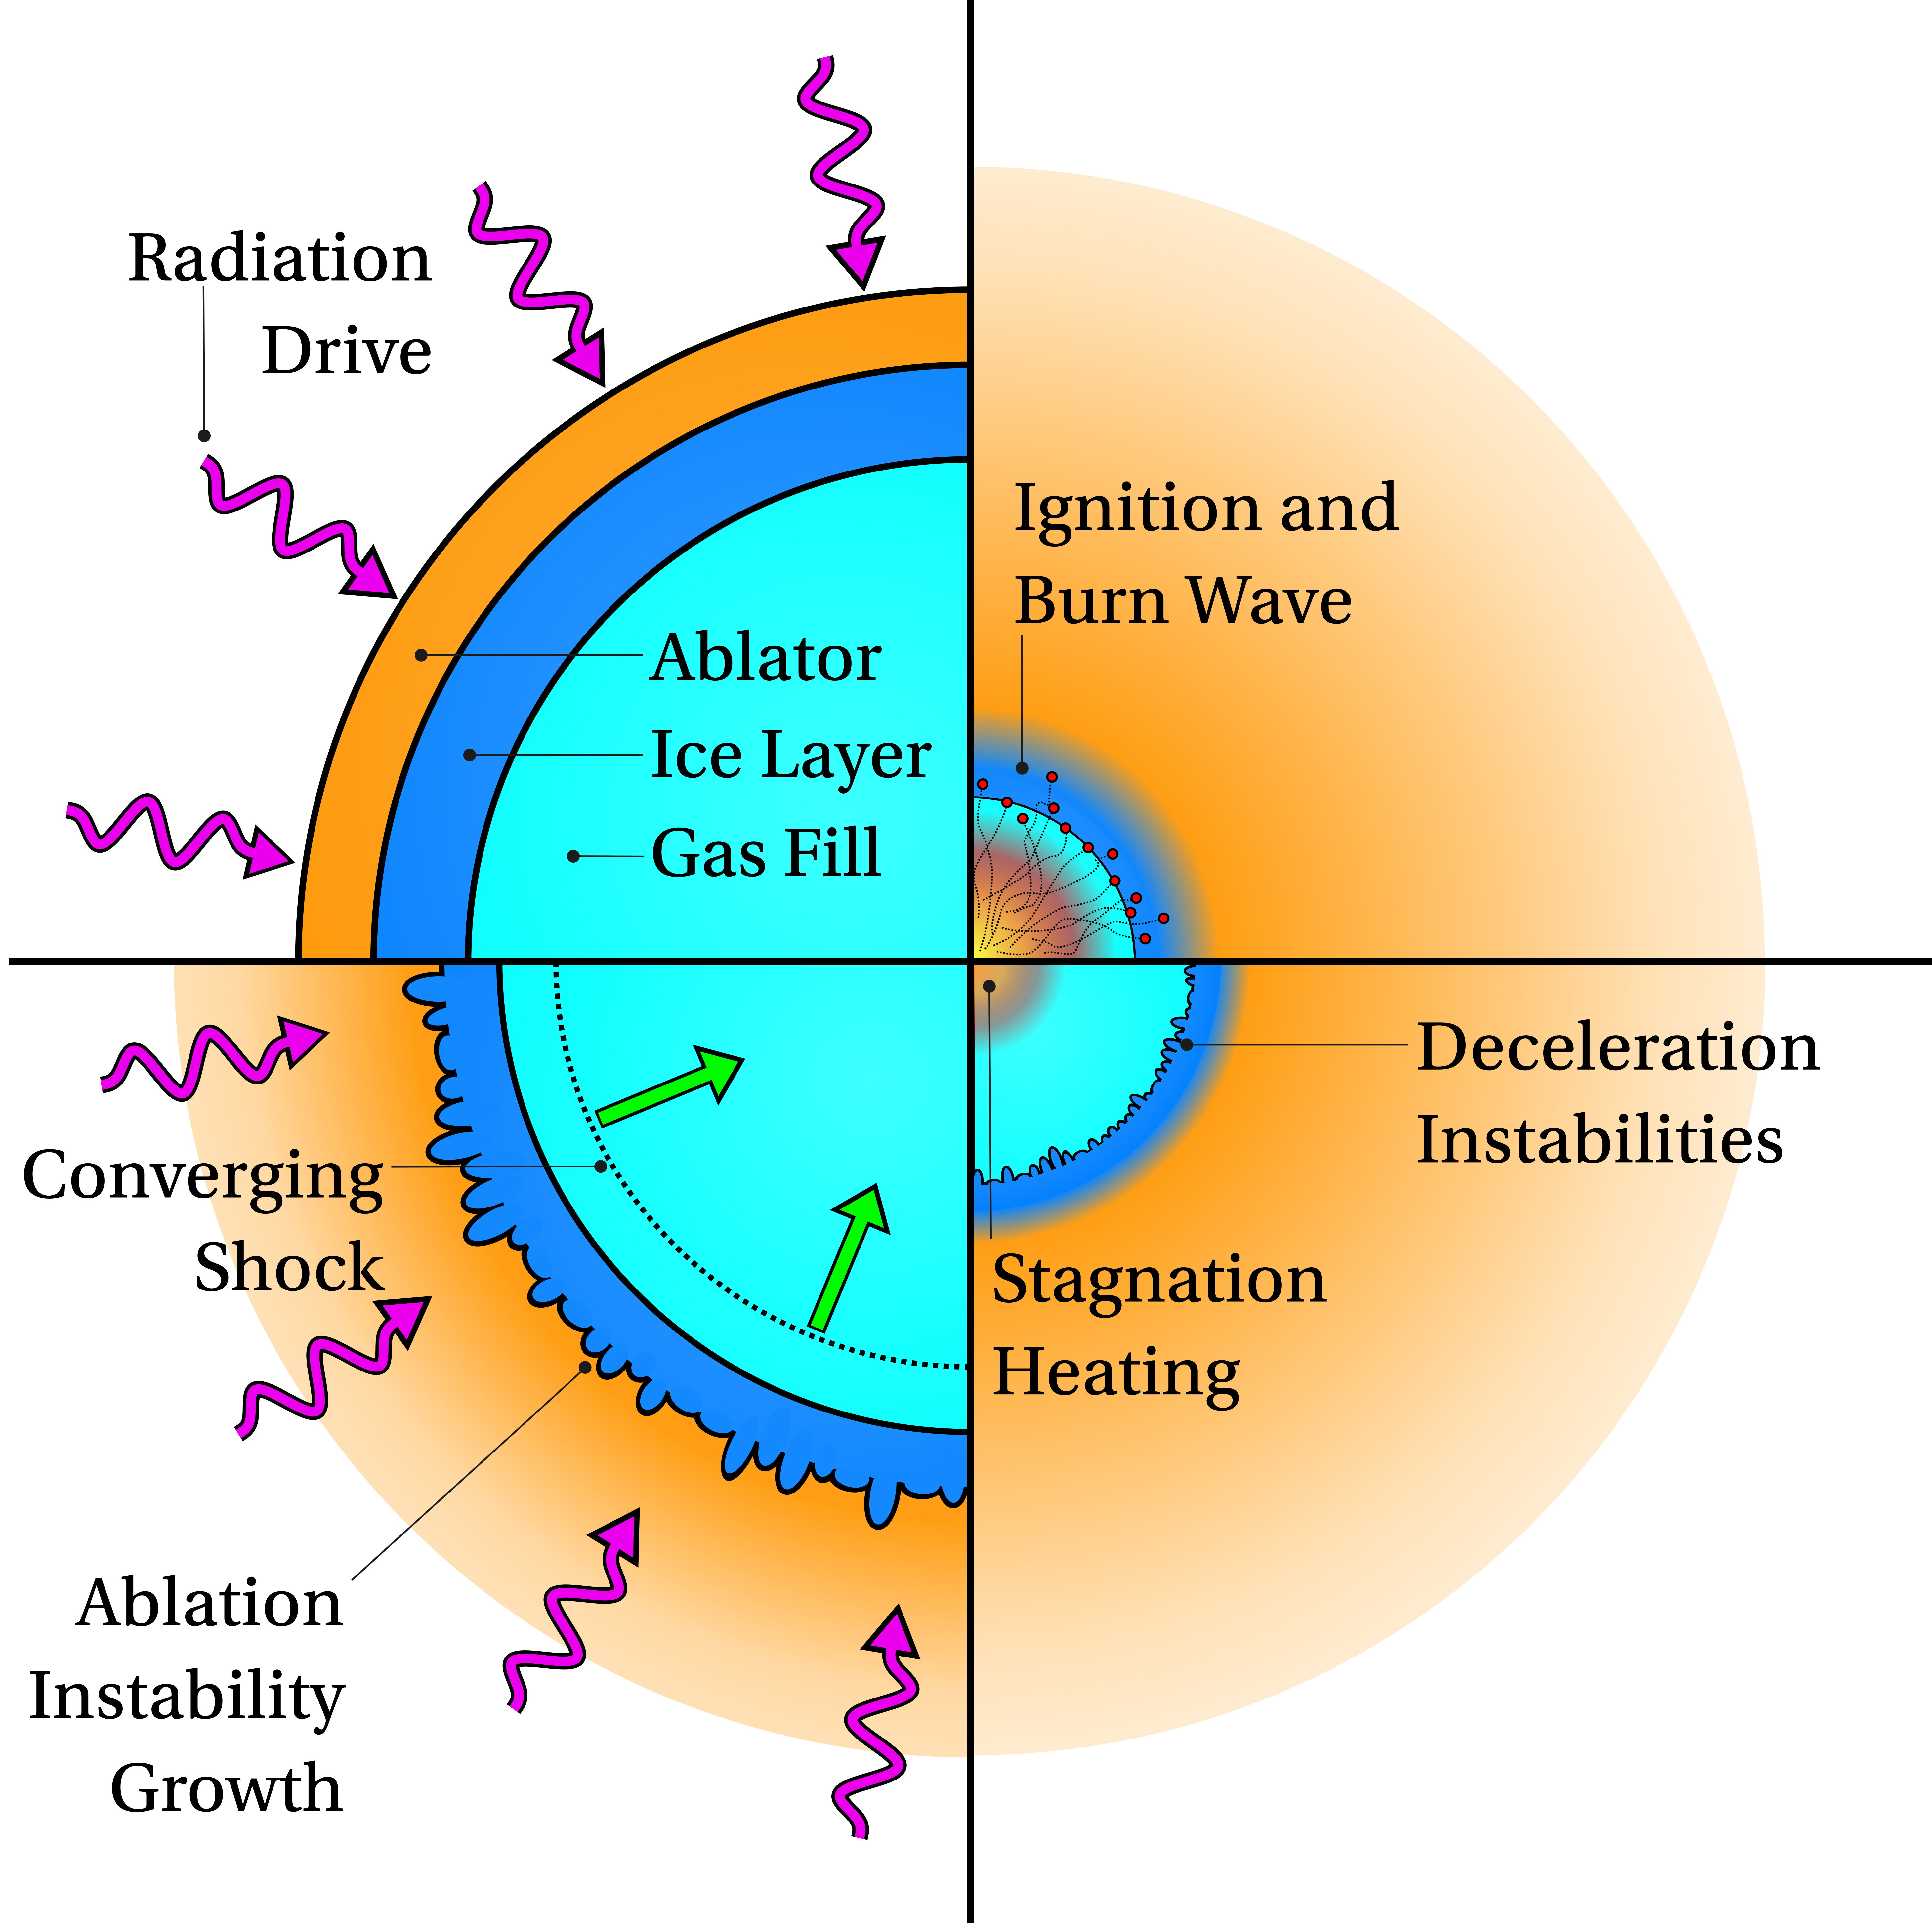
\includegraphics[width=0.7\linewidth]{Introduction/Images/hotspot ignition white.png}
    \centering
    \caption{Key Stages of the central hotspot ignition \ac{ICF} concept.
    }%
    \label{fig:intro_hotspot}
\end{figure}

Describe ablation pressure, ignite small volume of fuel etc.

%################################################################################
%################################################################################
\subsection{Alternative Approaches}%
\label{sec:intro_icf_alt}

Shock and fast ignition.

%################################################################################
%################################################################################
\subsection{Inertial Fusion Energy Considerations}%
\label{sec:intro_IFE_gain}

\begin{figure}[t!]
    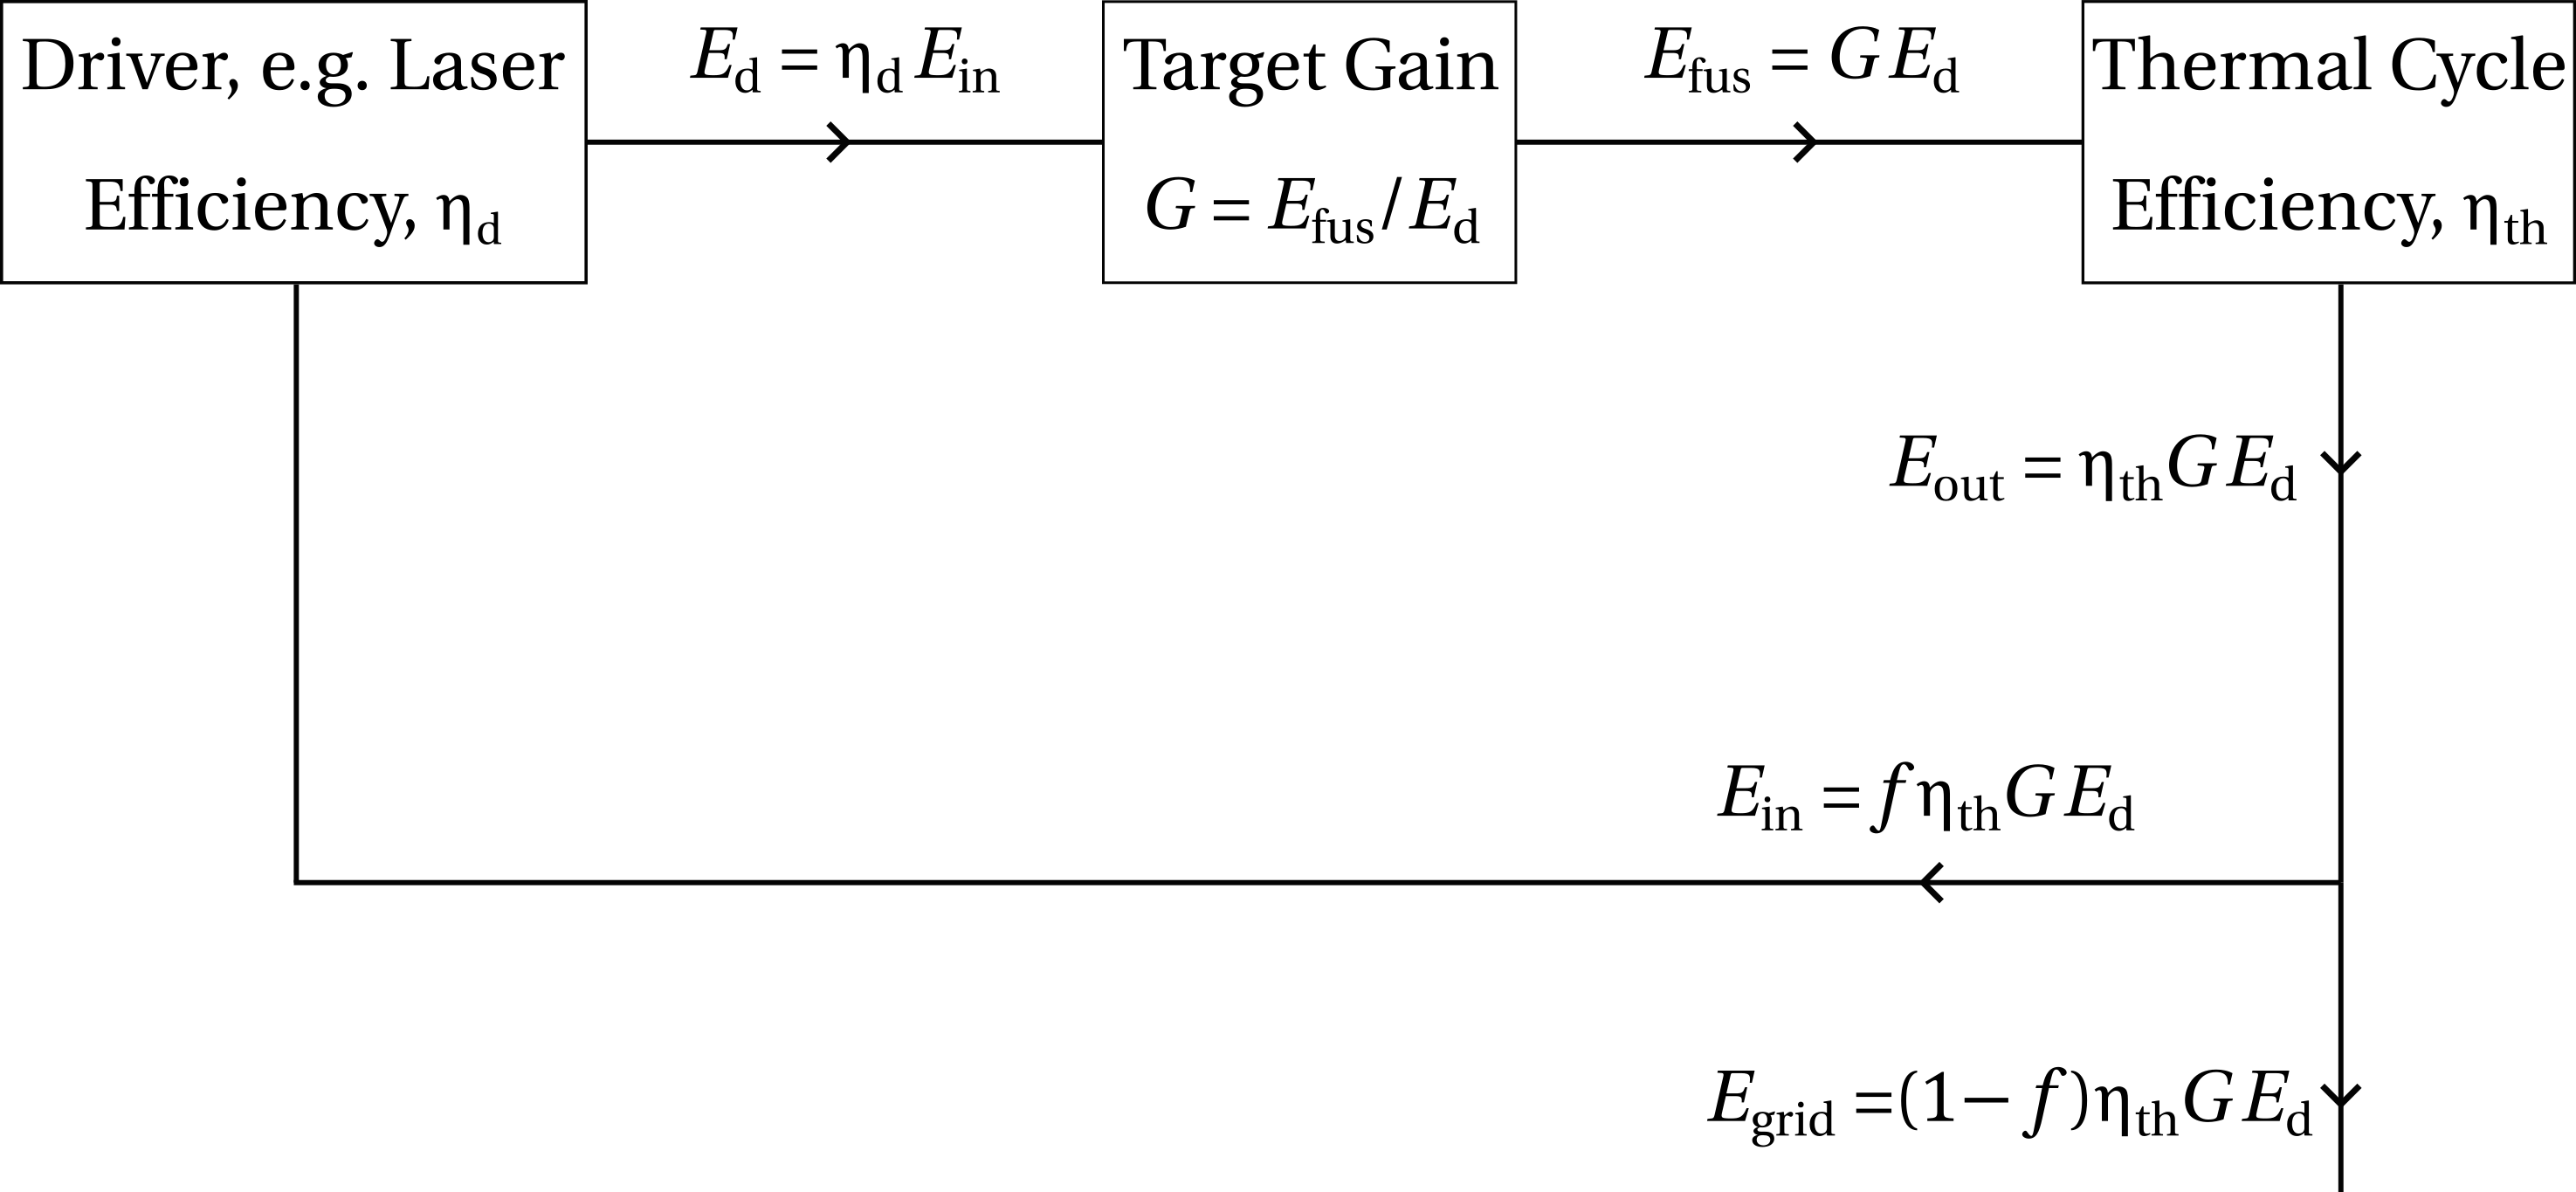
\includegraphics[width=0.8\linewidth]{Introduction/Images/IFE_powerplant.png}
    \centering
    \caption{Energy balance of an \ac{IFE} power plant.
    Based on a similar figure from Ref.~\cite{atzeni_physics_2004}.
    }%
    \label{fig:intro_IFE_energy_balance}
\end{figure}

For a power plant to produce net energy from \ac{ICF} implosions, the energy from each target must of course be greater than the energy to drive the implosion.
In reality, additional inefficiencies in power plants set more stringent constraints on the energy which must be produced.
The energy balance of an \ac{IFE} power plant is shown in Fig.~\ref{fig:intro_IFE_energy_balance}.
A driver, such as the lasers which are considered for the work conducted in this thesis, converts an input energy, $E_{\text{in}}$, to a driver energy, $E_{\text{d}} = \eta_{\text{d}}E_{\text{in}}$, where $\eta_{\text{d}}$ is the energy efficiency of the driver.
The driver energy initiates a fusion reaction, which releases energy $E_{\text{fus}}$, with gain, $G = E_{\text{fus}}/E_{\text{d}}$.
The released fusion energy, for example in the form of energetic neutrons, is converted into thermal energy in an encompassing `blanket', and then into output electrical energy, $E_\text{out}$ by a thermal-cycle (such as steam turbines), with efficiency, $\eta_{\text{th}}$.
Some fraction $f$ of this generated energy is recycled back into the plant to power the driver and the remaining fraction is sent to the grid,
\begin{equation}
    E_{\text{grid}} = (1-f) \eta_{\text{th}} \eta_{\text{d}} G E_{\text{in}},
\end{equation}
with the constraint, $f \eta_{\text{th}} \eta_{\text{d}} G \geq 1$ for net energy production.
Power plants must also produce a sufficiently large volume of energy to be economical.
Therefore, several $\sim100\ \text{MJ}$ reactions must occur each second for a $100 \text{MW}$ plant, which necessitates a driver that can operate at $\sim10\ \text{Hz}$.

The \ac{DPSSL} concept, could feasibly produce laser energy at $\sim10\ \text{Hz}$ repetition rate, with an efficiency $\eta_d\sim10\%$.
Assuming a thermal cycle efficiency, $\eta_{\text{th}}=40\%$ and a recycled energy fraction, $f=1/4$, this means that a target gain of approximately $G\sim100$ is required for power production.
Additionally, the plant must be economically profitable, thus for a $G=100$ reaction, which releases $E_{\text{fus}} = 100\ \text{MJ} = 28\ \text{kWh}$, the energy sold to the grid would make about $£1.50$\footnote{The UK April 2024 energy price of $£0.25$ per $\text{kWh}$ was used.}.
Therefore, targets must cost approximately $£0.10$, which limits the tolerable manufacturing complexity.
\ac{IFE} target concepts exist, which could feasibly be mass-produced for an acceptable cost, for example initially uniform density liquid spheres, known as `dynamic shell' targets~\cite{goncharov_novel_2020,igumenshchev_proof--principle_2023}.

%###############################################################################################################################
%###############################################################################################################################
%###############################################################################################################################
\section{Current Experiments/ Main Approaches}%
\label{sec:intro_mainexperiments}

Small intro on direct vs indirect.

%################################################################################
%################################################################################
\subsection{Indirect Drive}%
\label{sec:intro_indirect}

\begin{figure}[t!]
    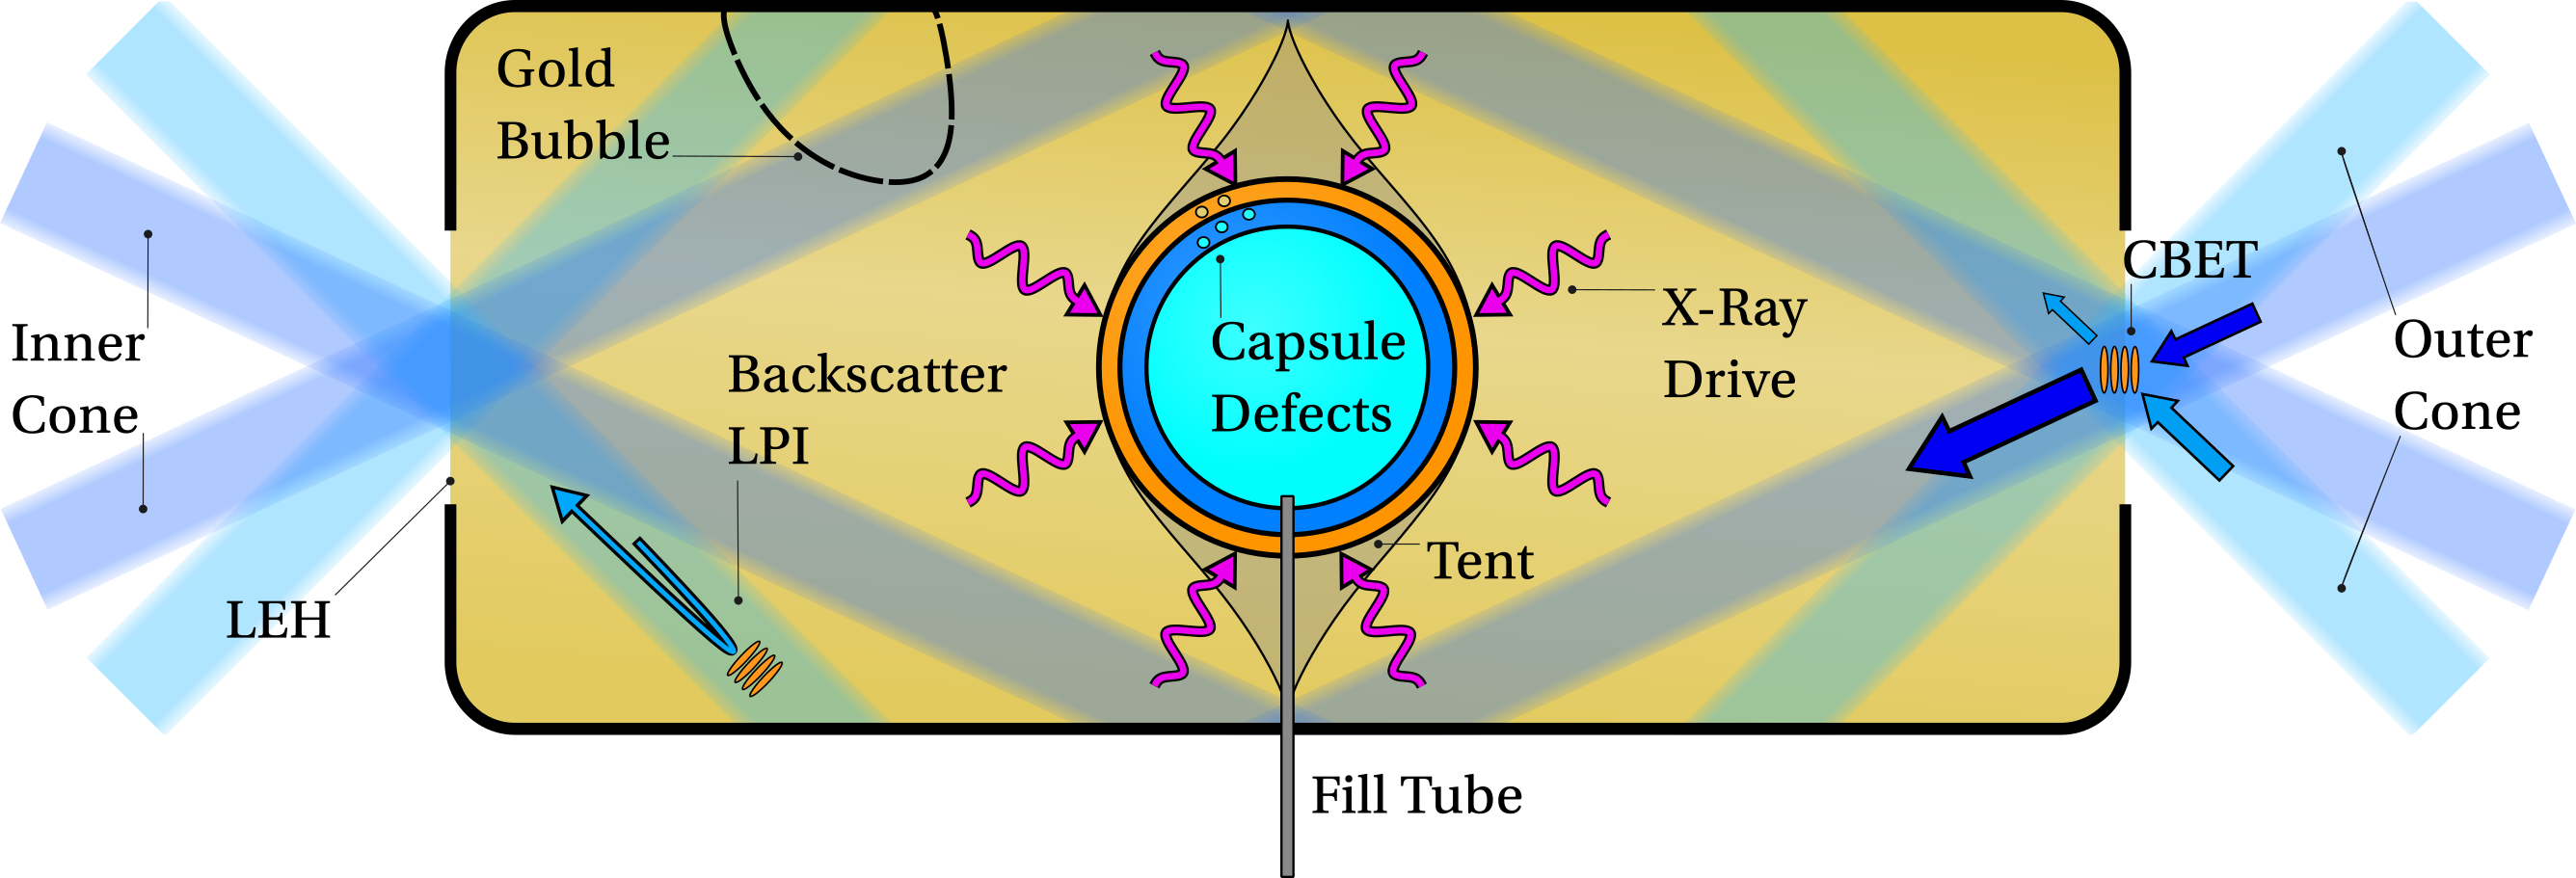
\includegraphics[width=\linewidth]{Introduction/Images/indirect icf white.png}
    \centering
    \caption{Schematic of the indirect-drive approach to \ac{ICF}.
    }%
    \label{fig:intro_indirect}
\end{figure}

Talk about all that jazz and give the diagram.
Talk about NIF and ignition, gain etc.

%################################################################################
%################################################################################
\subsection{Direct Drive}%
\label{sec:intro_direct}

\begin{figure}[t!]
    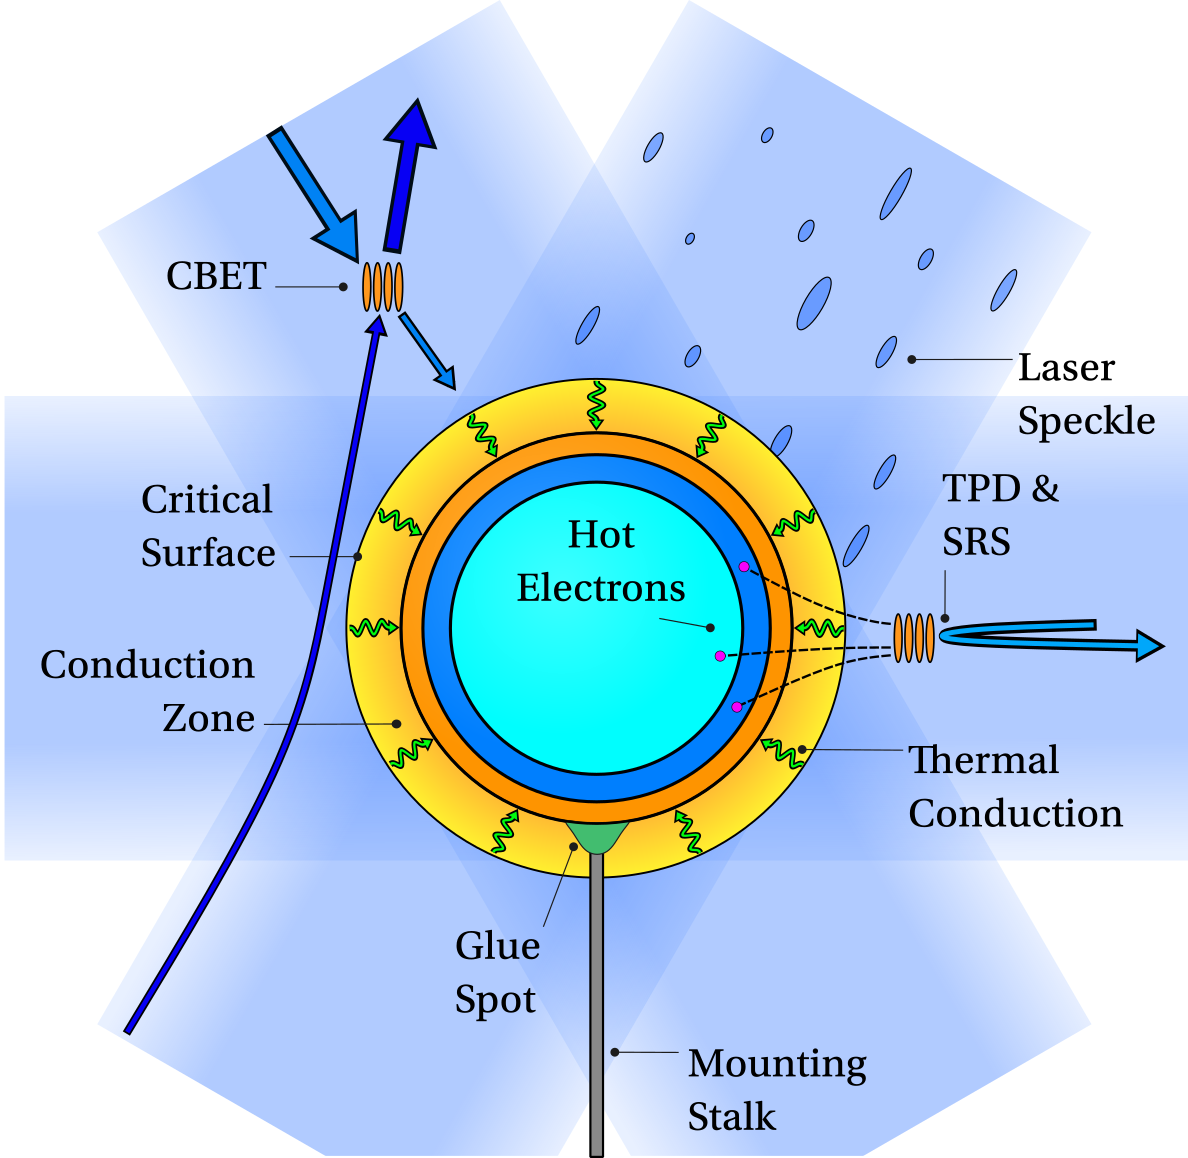
\includegraphics[width=0.7\linewidth]{Introduction/Images/direct icf white.png}
    \centering
    \caption{Schematic of the direct-drive approach to \ac{ICF}.
    }%
    \label{fig:intro_direct}
\end{figure}

Say its the assumed version for IFE.
Give a much more detailed anatomy of implosion, incl diagram.
Talk about hydro-scaled ignition etc.

%###############################################################################################################################
%###############################################################################################################################
%###############################################################################################################################
\section{Laser Interaction with Plasmas}%
\label{sec:intro_laserplasmas}

Understanding lasers is obviously crucial for Direct, indirect and hedp more generally.

%################################################################################
%################################################################################
\subsection{Regime of interest}%
\label{sec:intro_laser_regime}

Want collisional absorption and to avoid LPIs.
Therefore short wavelength, high power lasers, with limits to peak intensity.
Balance between $P_abl$ and high $I*lam^2$.

%################################################################################
%################################################################################
\subsection{ICF Relevant LPIs}%
\label{sec:intro_LPIs}

\begin{figure}[t!]
    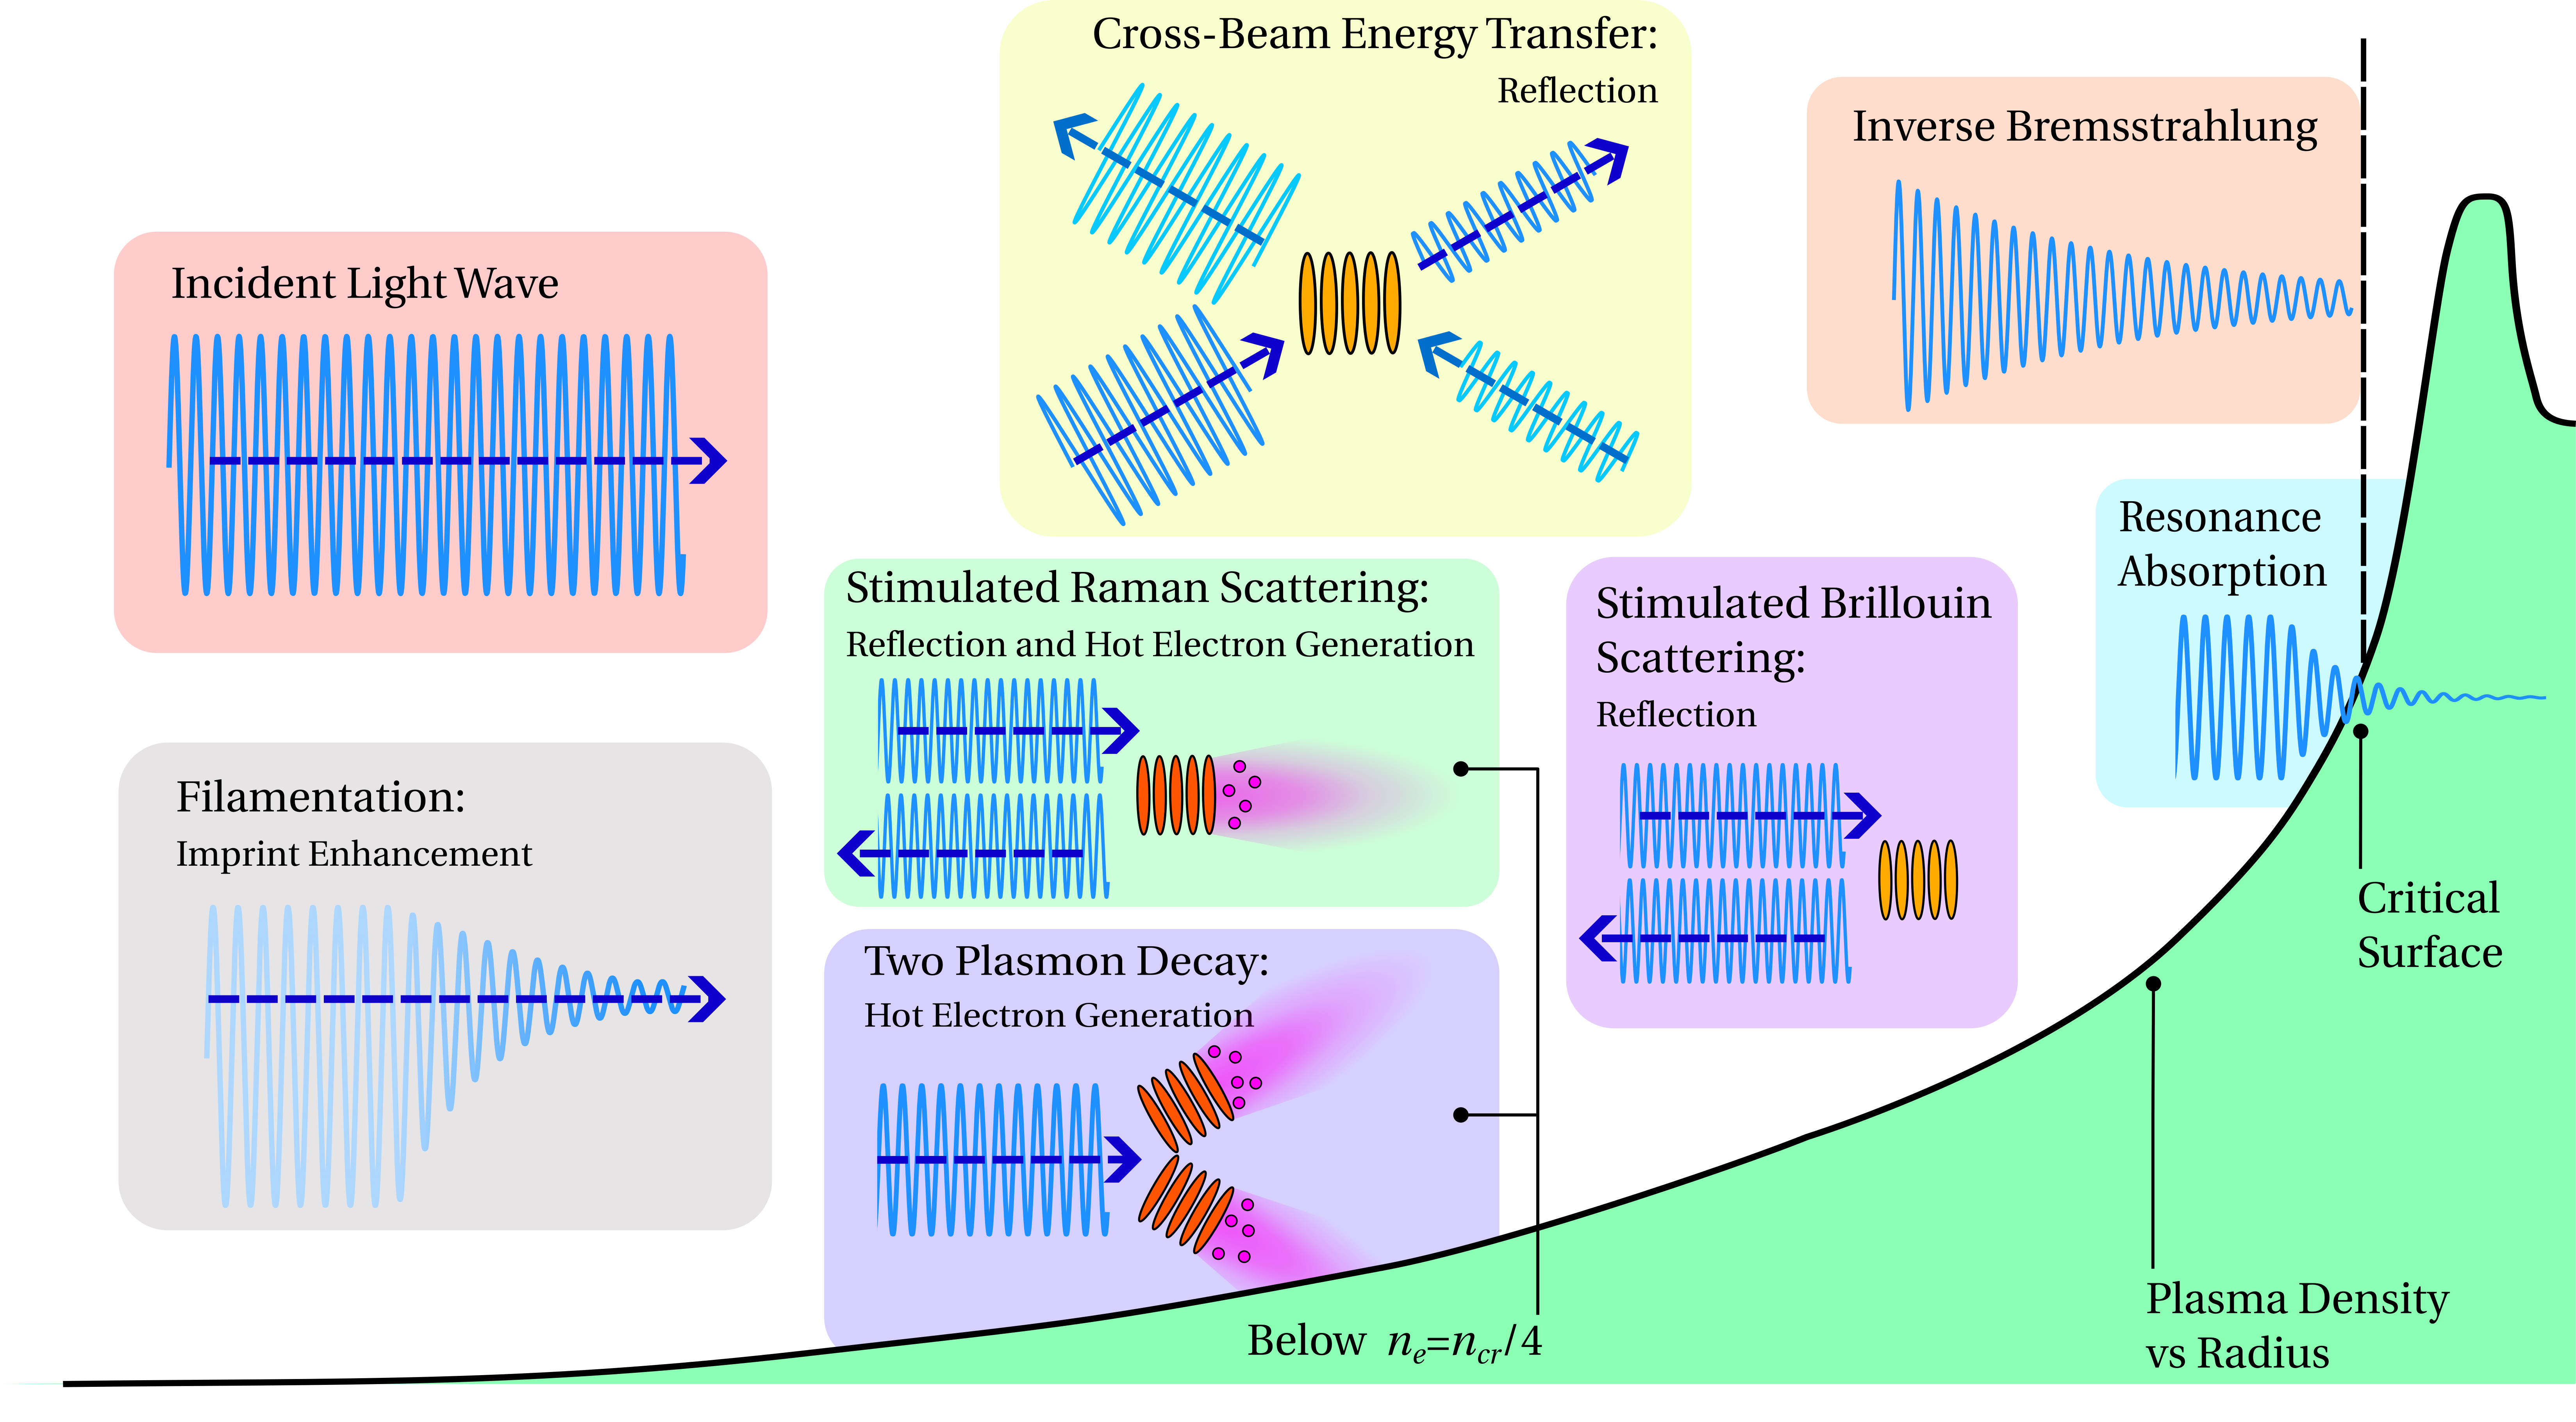
\includegraphics[width=\linewidth]{Introduction/Images/LPI diagram.png}
    \centering
    \caption{Important \ac{LPIs} for direct-drive \ac{ICF}.
    }%
    \label{fig:intro_dd_lpis}
\end{figure}

Damaging class of laser-plasma interactions for ICF.
Give diagram of how they work microphysically.
Include direct drive LPI diagram.
Introduce each in turn and say what they do for direct and indirect.

%###############################################################################################################################
%###############################################################################################################################
%###############################################################################################################################
\section{Objective of the work}%
\label{sec:intro_objective}

LPIs are important for current experiments.
Need to include models for them in integrated codes.
Also, next gen lasers will eliminate LPIs hopefully with bandwidth, so need to understand how they degrade current experiments to accurately extrapolate.
Create laser module for CHIMERA, specifically capable of modelling LPIs, and then see what their effect is for direct-drive.
